\documentclass{standalone}

\usepackage{tikz}
\usepackage{pgfplots}
\usetikzlibrary{calc, tikzmark, shapes, shapes.arrows, arrows, 3d, positioning}
\pgfplotsset{compat=1.17}
\begin{document}
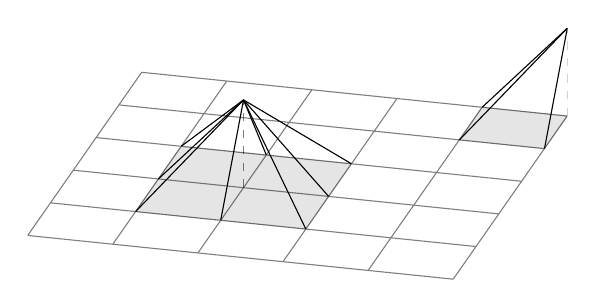
\begin{tikzpicture}
	\begin{axis}[anchor=origin, axis lines=none, xmin=-1, ymin=-1, xmax=4, ymax=4, zmin=-1, zmax=1.75, colormap/viridis, view={15}{35}]
		\begin{scope}[canvas is xy plane at z=0]
			\draw[opacity=.5] (-1,-1) grid (4,4); 
			\filldraw[opacity=.1] (0,0) rectangle (2,2); 
			\filldraw[opacity=.1] (3,3) rectangle (4,4);
		\end{scope}
		% \addplot3[domain=1:2, y domain=0:1, surf, opacity=0, fill opacity=.7, samples=30]({x},{y},{(2-x)*y}); 
		% \addplot3[domain=1:2, y domain=1:2, surf, opacity=0, fill opacity=.7, samples=30]({x},{y},{(2-x)*(2-y)}); 
		% \addplot3[domain=0:1, y domain=0:1, surf, opacity=0, fill opacity=.7, samples=30]({x},{y},{x*y}); 
		% \addplot3[domain=0:1, y domain=1:2, surf, opacity=0, fill opacity=.7, samples=30]({x},{y},{x*(2-y)}); 
		\draw[black, dashed, opacity=.5] (1,1,0) -- (1,1,1); 
		\draw[black] (0,0,0) -- (1,1,1); 
		\draw[black] (1,0,0) -- (1,1,1); 
		\draw[black] (2,0,0) -- (1,1,1); 
		\draw[black] (0,1,0) -- (1,1,1); 
		\draw[black] (2,1,0) -- (1,1,1); 
		\draw[black] (0,2,0) -- (1,1,1); 
		\draw[black] (1,2,0) -- (1,1,1); 
		\draw[black] (2,2,0) -- (1,1,1); 

		\draw[black] (4,3,0) -- (4,4,1); 
		\draw[black] (3,3,0) -- (4,4,1); 
		\draw[black] (3,4,0) -- (4,4,1); 
		\draw[black, dashed, opacity=.5] (4,4,0) -- (4,4,1); 
	\end{axis}
\end{tikzpicture}
\end{document}